\label{sec:data_acc_appendix}
\subsection{Publisher Denial of Service}
\label{sec:banning2}
As mentioned in \S\ref{sec:banning1}, Taylor \& Francis and ACS banned the scraping computer's IP address during the second stage of global scraping. This section explores why this occurred.

Taylor \& Francis banned the IP address after it detected over 100 requests were made within five minutes. This corresponds to a request every three seconds. This was a modest server load compared to other publishers, and was not foreseen to cause problems.

The ACS banning occurred because of a bug in the randomisation of requests. The program was instructed to take a DOI from a random publisher every time it made a request, rather than just a random DOI. Since the largest publisher was ACS, the program eventually exhausted DOIs from the other publishers, until there were only ACS DOIs to `randomly' draw requests from. This meant the request frequency to the ACS server went up dramatically. This increase broke the threshold of allowed requests at the ACS server which then banned the IP (approximately 10 requests a second).

\begin{figure}[H]
    \centering
    \textbf{ACS BANNING}\par\medskip
    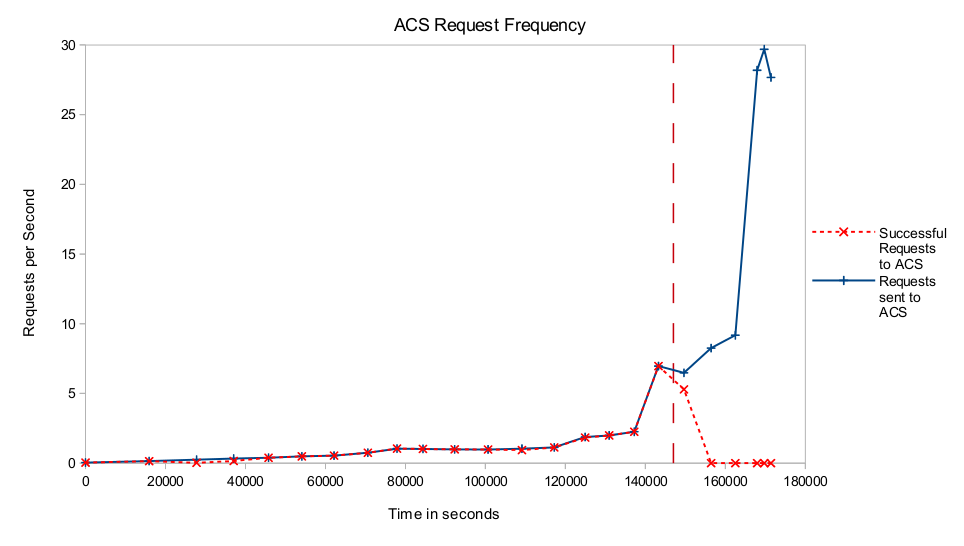
\includegraphics[width=0.9\textwidth]{Data_Acquisition/ACS_crash_line.png}
    \caption[Request Frequency Leading to ACS Ban]{The request frequency is plotted in blue, the received pages frequency in red. The vertical dashed line shows where the server detected the scape and banned the IP.}
     \label{fig:ACSBAN}
\end{figure}
The program was capable of making a total number of approximately 30 requests per second. As can be seen in figure \ref{fig:ACSBAN}, the program began to run out of requests to other publishers after approximately 140,000 seconds, resulting in an increase in the proportion of total requests per second to ACS. The ban occurred after approximately 150,000 seconds, after which there were no more responses received.

\subsection{Some Observations on $\Delta1$ through $\Delta6$}
\label{sec:CORPUSOBSERVATIONS}
There is much to be learnt by examination and simple statistics of the collected data. This section details some of this analysis which was used in development of the scraping program and to inform upon algorithm and processing design choices.

When deciding how many XPaths were required, it was necessary to examine publication profiles.
The publisher `market share' can be approximated from examining $\Delta3$.
\begin{figure}[H]
    \centering
    \textbf{Publisher Share in Chemistry Literature}\par\medskip
    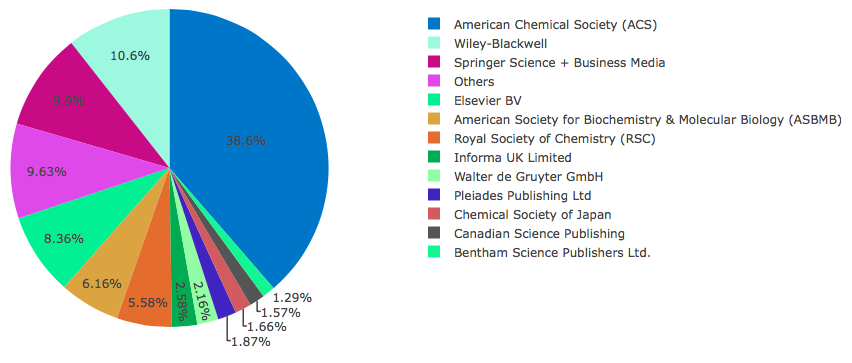
\includegraphics[width=\textwidth]{Data_Acquisition/publishers_pie3.png}
    \caption[Publisher Share in Chemistry Literature]{Articles grouped by publisher in $\Delta3$. Only the top 12 publishers are shown.}
     \label{fig:PUBPI}
\end{figure}
As shown in  shown in figure \ref{fig:PUBPI}, it can be seen that 90\% of all the chemistry literature collected was published by just 12 publishers, the majority from ACS, Wiley-Blackwell, Springer and Elsevier BV. Looking at the UK scraping DOI dataset (Figure \ref{fig:UKPUBPI}), the same large publishers are represented, but the Royal Society of Chemistry has a much larger share. This is to be expected, as the RSC is a UK based body. In the UK, there is a more even distribution between the large publishers. 

\begin{figure}[H]
    \centering
    \textbf{Publisher Share in UK Chemistry Literature}\par\medskip
    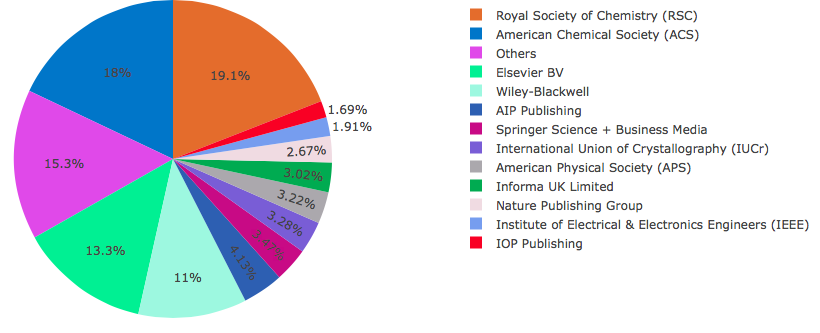
\includegraphics[width=\textwidth]{Data_Acquisition/uk_publishers_pie2.png}
    \caption[Publisher Share in UK Chemistry Literature]{Articles grouped by publisher in $\Delta1$. Only the top 12 publishers are shown.}
     \label{fig:UKPUBPI}
\end{figure}

The corpus of combined titles and abstracts in $\Delta6$ was then examined. An understanding of word distributions would inform data sanitiation practices. It is is included here for interes and completeness. The word frequencies across all the data were found to be approximately Zipfian, with a gradient of -1.11\footnote{A Zipfian distribution is a subset of the Pareto distribution, stating that the frequency of a word is proportional to its ranking in the word frequencies table. Ideally, the gradient of a log(frequency) vs log(rank) should be -1.0 \cite{zipf}} See figure \ref{fig:ZIPF}
\begin{figure}[H]
    \centering
    \textbf{Approximate Zipfian Distribution of Collected Corpus}\par\medskip
    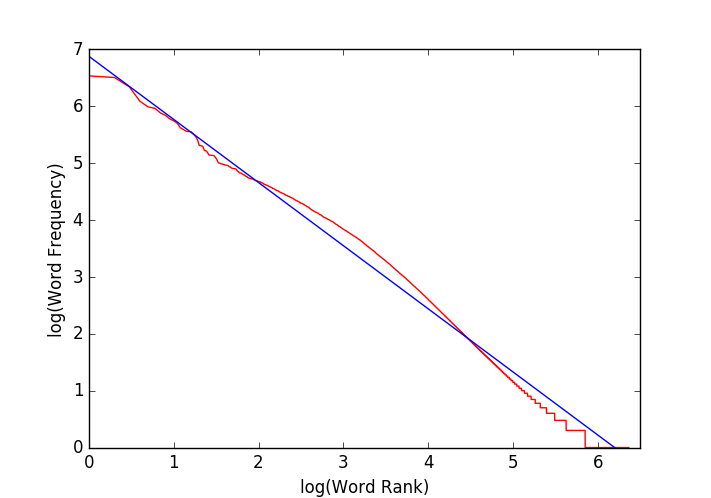
\includegraphics[scale=0.5]{Data_Acquisition/zipf.png}
    \caption[Zipfian Plot of Collected Corpus]{The log Frequency of words vs the log of their position in the rank in the word frequency table in blue. Best fit line in red, gradient = -1.11, intercept 6.3. }
     \label{fig:ZIPF}
\end{figure}
A summary of the corpus statistics are shown below:
\begin{table}[h!]
\caption{Titles and Abstracts in Databases}
\label{tab:CORPUS STATS}
\begin{center}
\begin{tabular}{||l|c|c||}
\hline
&$\Delta4$ (Global)& $\Delta2$ (UK)\\
\hline
Total Word Count & 61,296,410 & 2,256,722 \\
Total Unique Words & 2,326,725 & 60,166\\
Total Document Count & 464,712 & 16,363\\
Mode Words per Title &  11 & 11\\
Mean Words per Title &  12.2 & 14.0\\
Mode Words per Abstract & 156 & 52\\
Mean Words per Abstract & 119.7 & 158.4\\
Mode Sentences per Abstract & 4 & 4\\
Mean Sentences per Abstract & 5.4 & 6.0\\
\hline
\end{tabular}
\end{center}
\end{table}
Note that the mean scores are slightly higher for the UK, suggesting UK universities tend to publish slightly more verbose publications. The mode abstract length for the UK abstracts is significantly below the mean. This is indicative of a skewed, `noisy distribution', which is indeed found when the distribution is plotted (figure \ref{fig:abstract_sens}).
 \begin{figure}[H]
    \centering
    \textbf{Distribution of Abstract lengths in $\Delta2$ (articles from UK scrape)}\par\medskip
    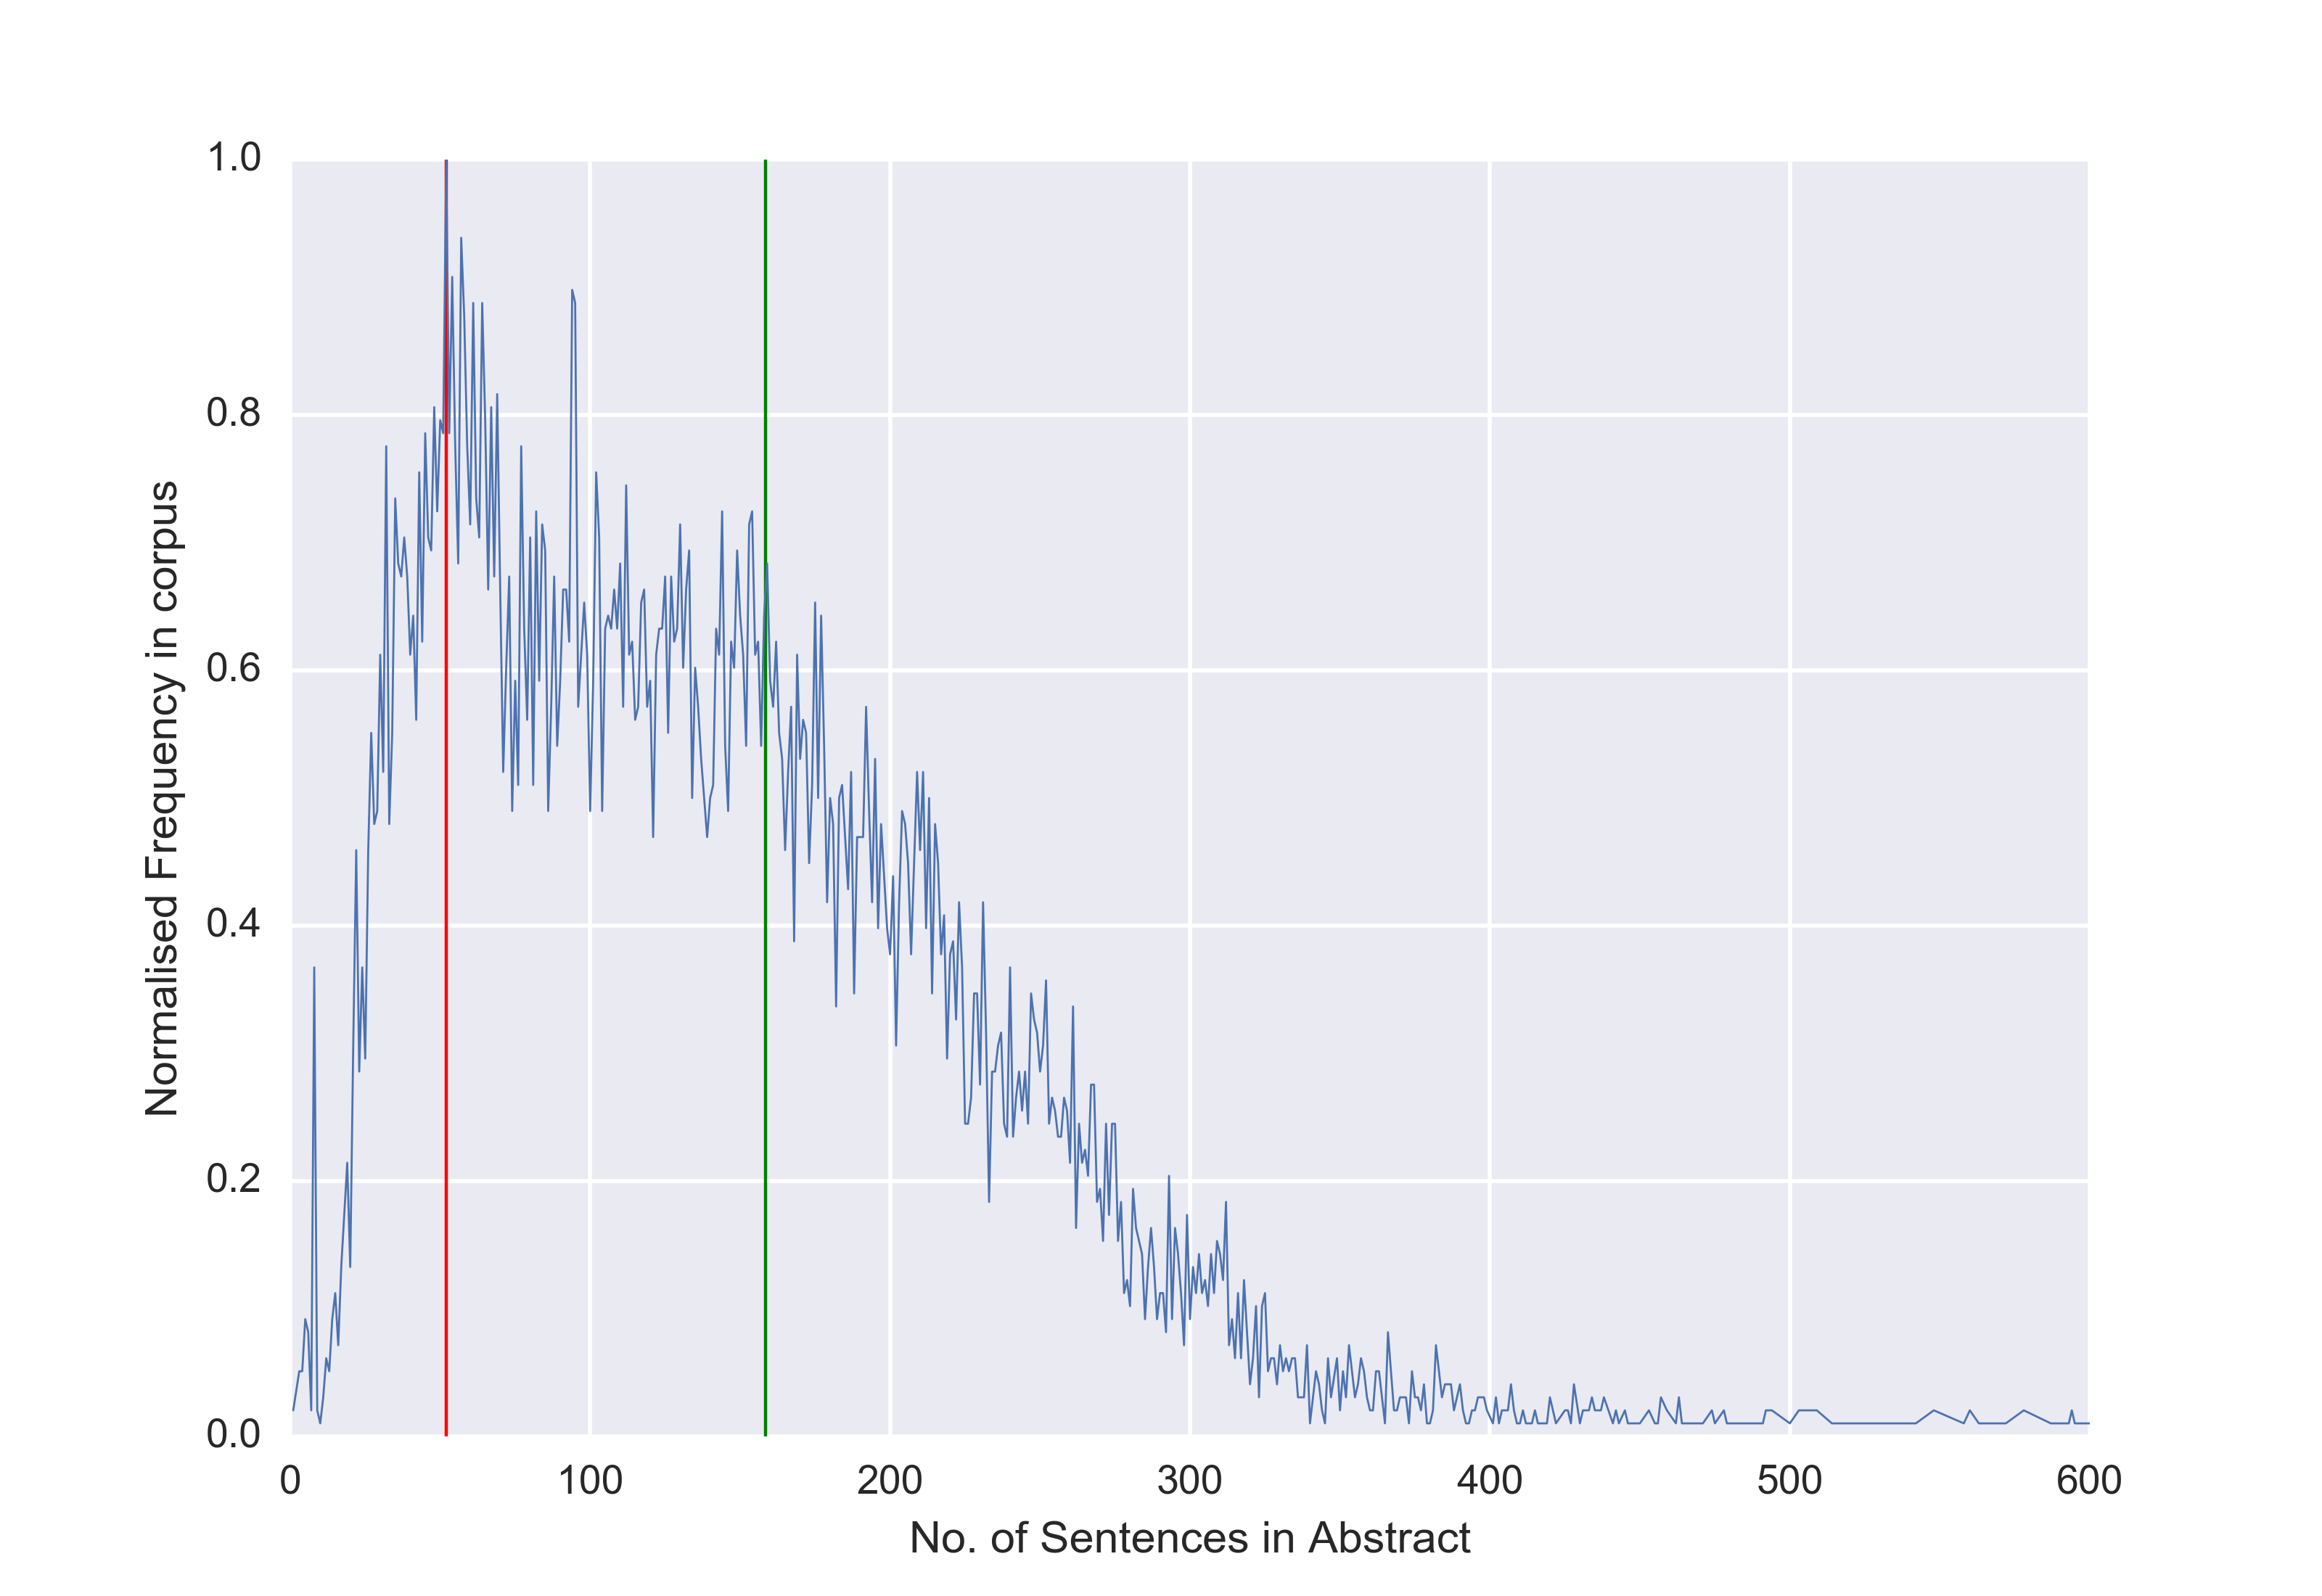
\includegraphics[width=0.8\textwidth]{Appendix/Data_Acquisition/abstracts.png}
    \caption[Distribution of Abstract lengths in $\Delta2$ (Articles from UK)]{Skewed distribution for number of words in abstracts. The mode is marked in red, the mean in green.}
     \label{fig:abstract_sens}
\end{figure}
As can be seen in the plot, there is significant variation in abstract lengths, with anything from 25 to 200 words commonly observed.
\label{sec:SCRAPEANALYSIS}


\subsection{UK Departments}
University Chemistry departments with suitable websites were considered when building the input list for the scraping program. Table \ref{tab:uk_scrape_depts} details all the departments that were included. A crawler program was written to navigate through these websites and store urls which had DOIs in them for the main program to scrape.
\begin{table}[H]
\caption{UK Chemistry Departments considered in Scraping}
\label{tab:uk_scrape_depts}
\begin{tabular}{||p{3.5cm}|W||}
\hline
 Department                         & URL \\
\hline
 \footnotesize{Aberdeen                       }    & \footnotesize{\url{www.abdn.ac.uk/chemistry/}}                                                                                                     \\
 \footnotesize{Aston                         }     & \footnotesize{\url{www.aston.ac.uk/eas/about-eas/academic-groups/ceac/}}                                                                           \\
 \footnotesize{Bangor                       }      & \footnotesize{\url{www.bangor.ac.uk/chemistry/index.php}}                                                                                          \\
 \footnotesize{Bath                        }       & \footnotesize{\url{www.bath.ac.uk/chemistry/}}                                                                                                     \\
 \footnotesize{Belfast (Queen's)          }        & \footnotesize{\url{www.qub.ac.uk/schools/SchoolofChemistryandChemicalEngineering/}}                                                                \\
\footnotesize{Birmingham                }         & \footnotesize{\url{www.birmingham.ac.uk/schools/chemistry/index.aspx}}                                                                             \\
\footnotesize{Bradford                 }          & \footnotesize{\url{www.brad.ac.uk/acad/chemistry/}                                                                                               } \\
 \footnotesize{Brighton                }           & \footnotesize{\url{about.brighton.ac.uk/pharmacy/}}                                                                                                \\
 \footnotesize{Bristol                }            & \footnotesize{\url{www.bris.ac.uk/Depts/Chemistry/Bristol\_Chemistry.html}}                                                                         \\
 \footnotesize{Cambridge             }             & \footnotesize{\url{www.ch.cam.ac.uk/}}                                                                                                             \\
 \footnotesize{Cardiff              }              & \footnotesize{\url{www.cardiff.ac.uk/chemistry}}                                                                                                   \\
 \footnotesize{Dundee              }               & \footnotesize{\url{www.lifesci.dundee.ac.uk}}                                                                                                      \\
 \footnotesize{Durham             }                & \footnotesize{\url{www.dur.ac.uk/chemistry/}}                                                                                                      \\
 \footnotesize{Edinburgh         }                 & \footnotesize{\url{www.chem.ed.ac.uk/}}                                                                                                            \\
 \footnotesize{Essex            }                  & \footnotesize{\url{www.essex.ac.uk/bs/}                                                                                                          } \\
 \footnotesize{Glasgow         }                   & \footnotesize{\url{www.chem.gla.ac.uk/}}                                                                                                           \\
 \footnotesize{Greenwich      }                    & \footnotesize{\url{www.gre.ac.uk/engsci/study/pharchemenv}}                                                                                        \\
 \footnotesize{Heriot-Watt   }                     & \footnotesize{\url{www.eps.hw.ac.uk/institutes/chemical-sciences.htm}}                                                                             \\
 \footnotesize{Hertfordshire}                      & \footnotesize{\url{www.herts.ac.uk/research/hhsri/research-areas-hhsri/pharmacy-and-pharmacology/pharmaceutical-chemistry}}                        \\
 \footnotesize{Huddersfield}                       & \footnotesize{\url{www.hud.ac.uk/sas/chemistry/}}                                                                                                  \\
 \footnotesize{Hull       }                        & \footnotesize{\url{www2.hull.ac.uk/science/chemistry.aspx}}                                                                                        \\
 \footnotesize{Keele     }                         & \footnotesize{\url{www.keele.ac.uk/chemistry/}}                                                                                                    \\
 \footnotesize{Kent Canterbury}                 & \footnotesize{\url{www.kent.ac.uk/bio/}}                                                                                                           \\
 \footnotesize{Kingston     }                      & \footnotesize{\url{sec.kingston.ac.uk/research/research-centres/}}                    
 \\
 \footnotesize{Lancaster   }                       & \footnotesize{\url{www.lancaster.ac.uk/chemistry/}}                                                                                                \\
\footnotesize{Leeds      }                        & \footnotesize{\url{www.chem.leeds.ac.uk/}}                                                                                                         \\
 \footnotesize{Leicester }                         & \footnotesize{\url{www.le.ac.uk/chemistry/}}                                                                                                                                                               
\\
\footnotesize{Lincoln                        }    & \footnotesize{\url{https://www.lincoln.ac.uk/home/chemistry/}}                                                                                            \\
 \footnotesize{Liverpool                     }     & \footnotesize{\url{www.liv.ac.uk/chemistry/}}                                                                                                      \\
 \footnotesize{Liverpool John Moores        }      & \footnotesize{\url{https://www.ljmu.ac.uk/about-us/faculties/faculty-of-science/school-of-pharmacy-and-biomolecular-sciences}}                            \\
 \footnotesize{London Met.         }       & \footnotesize{\url{www.londonmet.ac.uk/faculties/faculty-of-life-sciences-and-computing/school-of-human-sciences/}}                                
 \\
\hline 
 \end{tabular}
 \end{table}
 
 \begin{table}[H]
 \begin{tabular}{||p{4cm}|Y||}
\hline
 Department                         & URL \\
\hline
\footnotesize{Loughborough               }        & \footnotesize{\url{www.lboro.ac.uk/departments/chemistry}}                                                                                         \\
 \footnotesize{Manchester                }         & \footnotesize{\url{www.manchester.ac.uk/chemistry/}}                                                                                               \\
 \footnotesize{Manchester Met.  }          & \footnotesize{\url{www.sste.mmu.ac.uk}}                                                                                                            \\
 \footnotesize{Newcastle  }                        & \footnotesize{\url{www.ncl.ac.uk/chemistry/}}                                                                                                      \\
 \footnotesize{Northumbria}                        & \footnotesize{\url{https://www.northumbria.ac.uk/about-us/academic-departments/applied-sciences/}}\\
 \footnotesize{Nottingham                  }       & \footnotesize{\url{www.nottingham.ac.uk/chemistry/}}                                                                                               \\
 \footnotesize{Nottingham Trent}        & \footnotesize{\url{www.ntu.ac.uk/sat/about/academic\_teams/chemistry.html}}                                                                         \\
\footnotesize{ Open University }                   & \footnotesize{\url{www.open.ac.uk/science/chemistry/}}                                                                                             \\
 \footnotesize{Oxford}                             & \footnotesize{\url{www.chem.ox.ac.uk/}}                                                                                                            \\
 \footnotesize{Univ. West Scotland} & \footnotesize{\url{www.uws.ac.uk/schools/school-of-science/departments/chemistry-and-chemical-engineering/}}                                       \\
 \footnotesize{Plymouth               }            & \footnotesize{\url{https://www.plymouth.ac.uk/schools/school-of-geography-earth-and-environmental-sciences/chemistry}}                                    \\
\footnotesize{Reading               }             & \footnotesize{\url{www.reading.ac.uk/chemistry/}}                                                                                                  \\
 \footnotesize{Robert Gordon        }              & \footnotesize{\url{www.rgu.ac.uk/about/faculties-schools-and-departments/faculty-of-health-and-social-care/school-of-pharmacy-and-life-sciences1}} \\
 \footnotesize{St Andrews          }               & \footnotesize{\url{ch-www.st-and.ac.uk/}}                                                                                                          \\
 \footnotesize{Salford            }                & \footnotesize{\url{www.salford.ac.uk/environment-life-sciences/research/biomedical}}                                                               \\
 \footnotesize{Sheffield         }                 & \footnotesize{\url{www.sheffield.ac.uk/chemistry}}                                                                                                 \\
 \footnotesize{Sheffield Hallam }                  & \footnotesize{\url{www.shu.ac.uk/schools/sci/chem/}}                                                                                               \\
 \footnotesize{South Wales  }                      & \footnotesize{\url{www.southwales.ac.uk/chemistry/}}                                                                                               \\
 \footnotesize{Southampton }                       & \footnotesize{\url{www.soton.ac.uk/chemistry/}}                                                                                                    \\
 \footnotesize{Strathclyde}                        & \footnotesize{\url{www.strath.ac.uk/chemistry/}}                                                                                                   \\
 \footnotesize{Sunderland}                         & \footnotesize{\url{www.sunderland.ac.uk/ug/subjectareas/pharmacychemistrybiomedicalsciences/}}                                                     \\
 \footnotesize{Surrey }                            & \footnotesize{\url{www.surrey.ac.uk/chemistry/}}                                                                                                   \\
 \footnotesize{Sussex                            } & \footnotesize{\url{www.sussex.ac.uk/chemistry/}}                                                                                                   \\
 \footnotesize{Teesside                         }  & \footnotesize{\url{www.tees.ac.uk/schools/sst/}}                                                                                                   \\
 \footnotesize{UEA                             }   & \footnotesize{\url{www.uea.ac.uk/chemistry}}                                                                                                       \\
 \footnotesize{Warwick                        }    & \footnotesize{\url{www2.warwick.ac.uk/fac/sci/chemistry/}}                                                                                         \\
 \footnotesize{York                          }     & \footnotesize{\url{www.york.ac.uk/depts/chem/}}                                                                                                   \\ 
 \footnotesize{Bradford Ploymer IRC         }      & \footnotesize{\url{www.brad.ac.uk/acad/irc/}}                                                                                                      \\
 \footnotesize{Cardiff Pharmacy            }       & \footnotesize{\url{www.cardiff.ac.uk/pharmacy-pharmaceutical-sciences}}                                                                            \\
 \footnotesize{Burbeck Chemistry          }        & \footnotesize{\url{www.bbk.ac.uk/bcs/}}                                                                                                            \\
 \footnotesize{Burbeck Crystallography   }         & \footnotesize{\url{www.cryst.bbk.ac.uk/}}                                                                                                          \\
 \footnotesize{Imperial College London  }          & \footnotesize{\url{www.imperial.ac.uk/chemistry/}}                                                                                                 \\
 \footnotesize{King's College London   }          & \footnotesize{\url{www.kcl.ac.uk/nms/depts/chemistry/index.aspx}}                                                                                  \\
 \footnotesize{Queen Mary London      }            & \footnotesize{\url{www.sbcs.qmul.ac.uk/}}                                                                                                          \\
 \footnotesize{UCL School of Pharmacy}             & \footnotesize{\url{www.ucl.ac.uk/pharmacy}}                                                                                                        \\
 \footnotesize{University College London}          & \footnotesize{\url{www.ucl.ac.uk/chemistry/}}                                                                                                      \\
 \footnotesize{Sheffield Comput. Chem.}  & \footnotesize{\url{www.sheffield.ac.uk/is/research/groups/chemoinformatics}}   
 \\
 \hline
\end{tabular}
\end{table}

\subsection{Publishers Considered in UK scraping}
The UK scraping run found articles published by 36 different publishers. These are detailed below in table \ref{tab:uk_publishers_table}.
\begin{table}[H]
\centering
\caption{All publishers found in the UK scraping run}
\label{tab:uk_publishers_table}
\begin{tabular}{||c||}
\hline 
IBM                                               \\
Pleiades Publishing Ltd                           \\
Informa Healthcare                                \\
Informa UK Limited                                \\
Royal Society of Chemistry (RSC)                  \\
Vilnius Gediminas Technical University            \\
Technical Association of Photopolymers, Japan     \\
Springer US                                       \\
Trans Tech Publications                           \\
Thieme Publishing Group                           \\
Nature Publishing Group                           \\
American Physical Society (APS)                   \\
IOP Publishing                                    \\
Institute of Electrical \& Electronics Engineers (IEEE)\\
American Chemical Society (ACS)                   \\
Walter de Gruyter GmbH                            \\
Pharmaceutical Society of Japan                   \\
American Association of Physics Teachers (AAPT)   \\
AIP Publishing                                    \\
Japan Society of Applied Physics                  \\
American Vacuum Society                           \\
Wiley-Blackwell                                   \\
Springer Berlin Heidelberg                        \\
Springer New York                                 \\
Royal Society of Chemistry                        \\
Public Library of Science (PLoS)                  \\
Surface Science Society Japan                     \\
Springer Science + Business Media                 \\
The Royal Society                                 \\
Society of Rheology                               \\
Acoustical Society of America (ASA)               \\
Springer International Publishing                 \\
Proceedings of the National Academy of Sciences   \\
Japan Society for Analytical Chemistry            \\
International Union of Crystallography (IUCr)     \\
Chemical Society of Japan                         \\
EDP Sciences                                      \\
\hline
\end{tabular}
\end{table}

